\documentclass{ximera}

\newcommand{\RR}{\mathbb R}
\renewcommand{\d}{\,d}
\newcommand{\dd}[2][]{\frac{d #1}{d #2}}
\renewcommand{\l}{\ell}
\newcommand{\ddx}{\frac{d}{dx}}
\newcommand{\dfn}{\textbf}
\newcommand{\eval}[1]{\bigg[ #1 \bigg]}


\author{Jim Talamo and Bart Snapp}
\license{Creative Commons 3.0 By-NC}


\outcome{Compute integrals involving powers of sine and cosine}
\outcome{Recognize the patterns that appear in trigonometric integrals,
  and use appropriate substitutions to compute them.}


\begin{document}
\begin{exercise}

This exercise explores a general method of integrating products of $\sin(x)$ and $\cos(x)$ when the power of $\sin(x)$ is odd.  For any odd integer, we can find an integer $k$ so that the original odd integer takes the form $2k+1$.  For instance:

\begin{exercise}
If our original odd integer is $7$, we can express $7 = 2 \cdot \answer{3}+1$, so $k=\answer{3}$.

If our original odd integer is $93$, we can express $93 = 2 \cdot \answer{41}+1$, so $k=\answer{41}$.
\end{exercise}

 If we are integrating a product of powers of sine and cosine functions, and the power of sine is odd, then the integral looks like
\[
\int \sin^{2k+1}(x) \cos^m(x) \d x
\]
where $k$ and $m$ are integers.  Then:

\begin{align*}
  \int \sin^{2k+1}(x) \cos^m(x) \d x &=\int(\sin^{2}(x))^2 \cos^m(x) \sin(x) \d x\\
  &= \int (1-\cos^2(x))^2 \cos^m(x) \sin(x)\d x.
\end{align*}
We have now set ourselves up for an eventual substitution:
\begin{center}%% used center instead of image since there is no reason for a LARGE integral in the text
  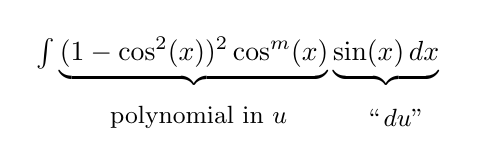
\begin{tikzpicture}
    \node at (0,0) {
      $\int \underbrace{(1-\cos^2(x))^2 \cos^m(x)} \underbrace{\sin(x) \d x}$
        };
    \node at (-.5,-.7) {\small{polynomial in $u$}};
    \node at (2,-.7) {\small{``$\d u$''}};
  \end{tikzpicture}
\end{center}
so letting $u = \cos(x)$ so $\d u =\answer{-\sin(x)} \d x$, we have
\[
  \int \sin^{2k+1}(x) \cos^m(x) \d x =\int(\sin^{2}(x))^2 \cos^m(x) \sin(x) \d x = \int -(1-u^2)^2 u^m \d u
\]
which is a polynomial, and can be integrated term-by-term after expansion.

Of course, this was quite general, and a real example is worth a thousand generalities:

\begin{exercise}
We find $\int \sin^5(x) \cos^4(x) \d x$ by following the above prototype.  Here we have:

\[
\int \sin^{2k+1}(x) \cos^m(x) \d x
\]
and can find that $k=\answer{2}$ and $m=\answer{4}$.

\begin{align*}
  \int \sin^{2k+1}(x) \cos^4(x) \d x &=  \int \sin^{2(2)+1}(x) \cos^4(x) \d x \\
  &= \int(\sin^{2}(x))^2 \cos^4(x) \sin(x) \d x\\
  &= \int (1-\cos^2(x))^2 \cos^4(x) \sin(x)\d x.
\end{align*}
We have now set ourselves up for an eventual substitution:
\begin{center}%% used center instead of image since there is no reason for a LARGE integral in the text
  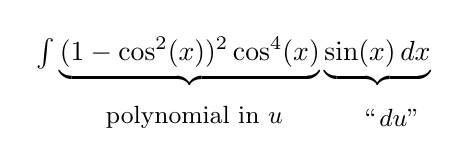
\begin{tikzpicture}
    \node at (0,0) {
      $\int \underbrace{(1-\cos^2(x))^2 \cos^4(x)} \underbrace{\sin(x) \d x}$
        };
    \node at (-.5,-.7) {\small{polynomial in $u$}};
    \node at (2,-.7) {\small{``$\d u$''}};
  \end{tikzpicture}
\end{center}
so letting $u = \cos(x)$ so $\d u =\answer{-\sin(x)} \d x$, we have
\[
\int -(1-u^2)^2 u^4 \d u
\]
which is a polynomial, and can be integrated term-by-term after expansion.  

\begin{exercise}
We can now perform this expansion since we have actual constants to find:

\[  \int(\sin^{2}(x))^2 \cos^4(x) \sin(x) \d x = \int -u^8+2u^6-u^4 \d u =\answer{-\frac{1}{9}u^9+\frac{2}{7}u^7-\frac{1}{5}u^5 +C}\]

(Use $C$ for the constant of integration and express your antiderivative in terms of $u$)
\begin{exercise}

Reversing the substitution gives:

\[
\int \sin^5(x) \cos^4(x) \d x=\answer{-\frac{1}{9}\sin^9(x)+\frac{2}{7}\sin^7(x)-\frac{1}{5}\sin^5(x) +C}
\]
\end{exercise}


\end{exercise}
\end{exercise}
\end{exercise}
\end{document}
